\documentclass[14pt]{extbook}
\usepackage{multicol, enumerate, enumitem, hyperref, color, soul, setspace, parskip, fancyhdr} %General Packages
\usepackage{amssymb, amsthm, amsmath, latexsym, units, mathtools} %Math Packages
\everymath{\displaystyle} %All math in Display Style
% Packages with additional options
\usepackage[headsep=0.5cm,headheight=12pt, left=1 in,right= 1 in,top= 1 in,bottom= 1 in]{geometry}
\usepackage[usenames,dvipsnames]{xcolor}
\usepackage{dashrule}  % Package to use the command below to create lines between items
\newcommand{\litem}[1]{\item#1\hspace*{-1cm}\rule{\textwidth}{0.4pt}}
\pagestyle{fancy}
\lhead{Progress Quiz 6}
\chead{}
\rhead{Version C}
\lfoot{4563-7456}
\cfoot{}
\rfoot{Summer C 2021}
\begin{document}

\begin{enumerate}
\litem{
Graph the equation below.\[ f(x) = -(x+2)^2 - 16 \]\begin{enumerate}[label=\Alph*.]
\begin{multicols}{2}\item 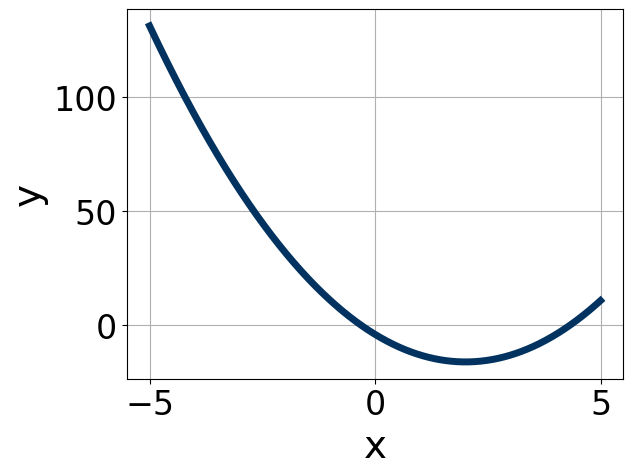
\includegraphics[width = 0.3\textwidth]{../Figures/quadraticEquationToGraphCopyAC.png}\item 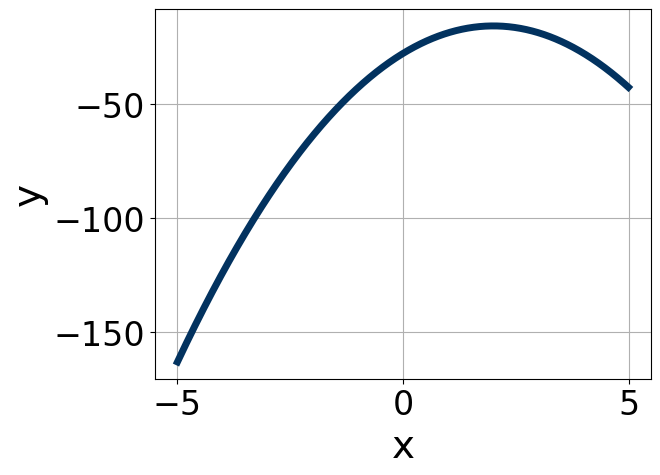
\includegraphics[width = 0.3\textwidth]{../Figures/quadraticEquationToGraphCopyBC.png}\item 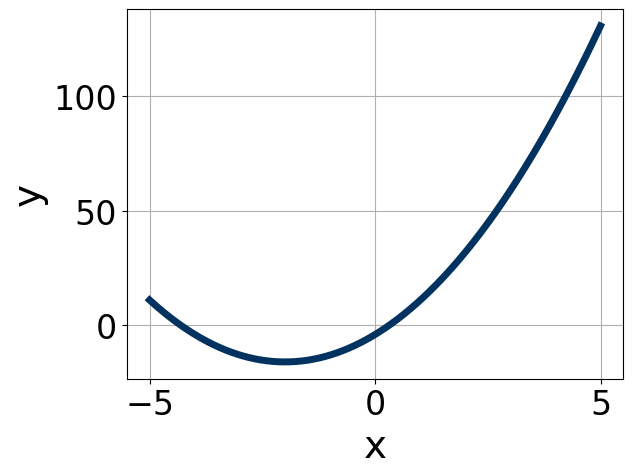
\includegraphics[width = 0.3\textwidth]{../Figures/quadraticEquationToGraphCopyCC.png}\item 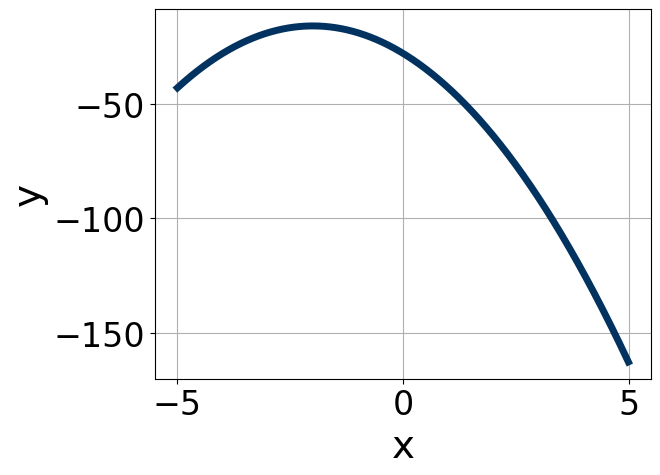
\includegraphics[width = 0.3\textwidth]{../Figures/quadraticEquationToGraphCopyDC.png}\end{multicols}\item None of the above.
\end{enumerate} }
\litem{
Factor the quadratic below. Then, choose the intervals that contain the constants in the form $(ax+b)(cx+d); b \leq d.$\[ 36x^{2} +61 x + 20 \]\begin{enumerate}[label=\Alph*.]
\item \( a \in [7, 14], \hspace*{5mm} b \in [4, 5], \hspace*{5mm} c \in [3.26, 4.33], \text{ and } \hspace*{5mm} d \in [3, 9] \)
\item \( a \in [-3, 2], \hspace*{5mm} b \in [15, 19], \hspace*{5mm} c \in [-0.27, 1.45], \text{ and } \hspace*{5mm} d \in [41, 52] \)
\item \( a \in [3, 8], \hspace*{5mm} b \in [4, 5], \hspace*{5mm} c \in [7.89, 8.53], \text{ and } \hspace*{5mm} d \in [3, 9] \)
\item \( a \in [27, 29], \hspace*{5mm} b \in [4, 5], \hspace*{5mm} c \in [-0.27, 1.45], \text{ and } \hspace*{5mm} d \in [3, 9] \)
\item \( \text{None of the above.} \)

\end{enumerate} }
\litem{
Factor the quadratic below. Then, choose the intervals that contain the constants in the form $(ax+b)(cx+d); b \leq d.$\[ 24x^{2} -10 x -25 \]\begin{enumerate}[label=\Alph*.]
\item \( a \in [7.89, 8.65], \hspace*{5mm} b \in [-8, -4], \hspace*{5mm} c \in [1.8, 4.8], \text{ and } \hspace*{5mm} d \in [1, 6] \)
\item \( a \in [-1.13, 1.53], \hspace*{5mm} b \in [-30, -28], \hspace*{5mm} c \in [0.5, 1.7], \text{ and } \hspace*{5mm} d \in [19, 23] \)
\item \( a \in [2.93, 4.07], \hspace*{5mm} b \in [-8, -4], \hspace*{5mm} c \in [4.8, 8.9], \text{ and } \hspace*{5mm} d \in [1, 6] \)
\item \( a \in [1.83, 3.68], \hspace*{5mm} b \in [-8, -4], \hspace*{5mm} c \in [11.5, 14.6], \text{ and } \hspace*{5mm} d \in [1, 6] \)
\item \( \text{None of the above.} \)

\end{enumerate} }
\litem{
Graph the equation below.\[ f(x) = (x+1)^2 - 17 \]\begin{enumerate}[label=\Alph*.]
\begin{multicols}{2}\item 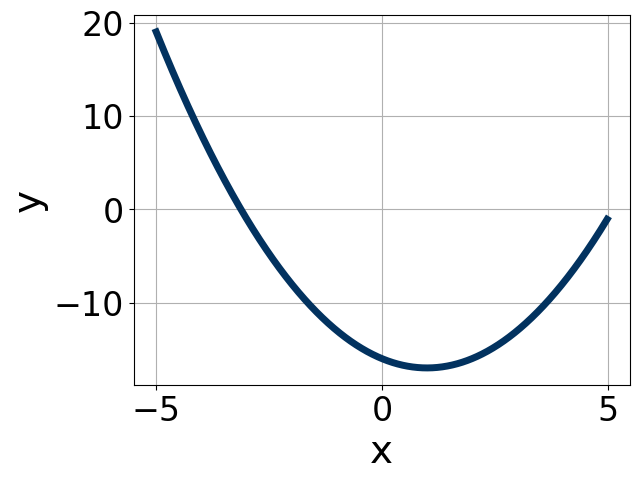
\includegraphics[width = 0.3\textwidth]{../Figures/quadraticEquationToGraphAC.png}\item 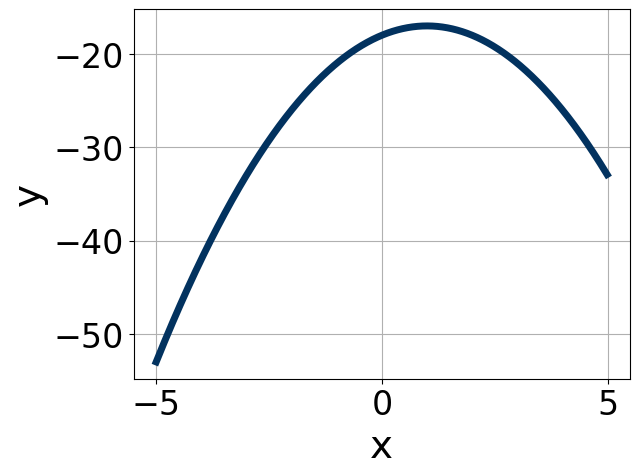
\includegraphics[width = 0.3\textwidth]{../Figures/quadraticEquationToGraphBC.png}\item 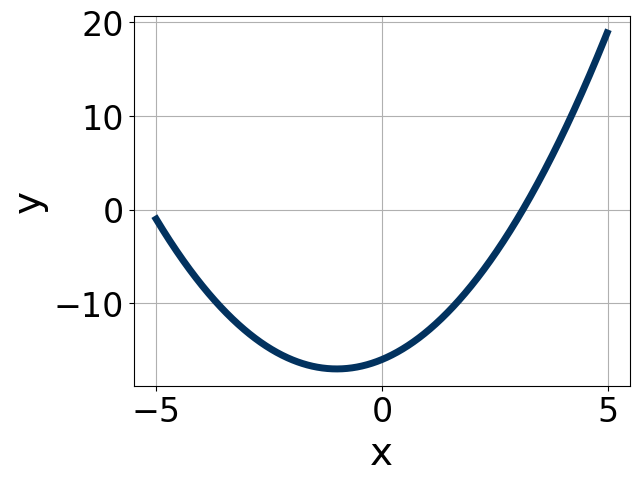
\includegraphics[width = 0.3\textwidth]{../Figures/quadraticEquationToGraphCC.png}\item 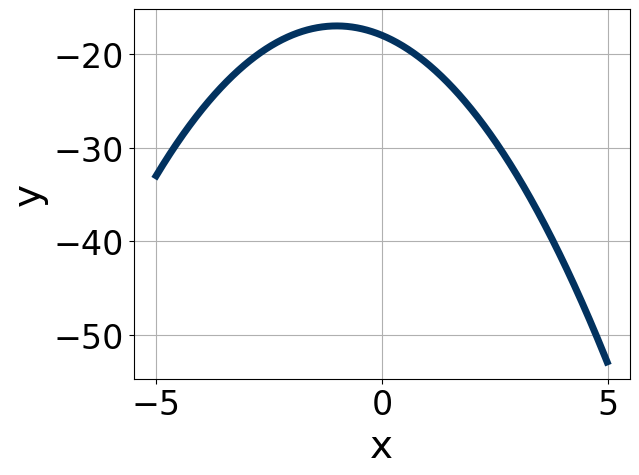
\includegraphics[width = 0.3\textwidth]{../Figures/quadraticEquationToGraphDC.png}\end{multicols}\item None of the above.
\end{enumerate} }
\litem{
Solve the quadratic equation below. Then, choose the intervals that the solutions belong to, with $x_1 \leq x_2$ (if they exist).\[ 14x^{2} -11 x -8 = 0 \]\begin{enumerate}[label=\Alph*.]
\item \( x_1 \in [-7.7, -6.2] \text{ and } x_2 \in [16.4, 19.3] \)
\item \( x_1 \in [-1.5, -1.1] \text{ and } x_2 \in [-1.2, 1.1] \)
\item \( x_1 \in [-0.9, -0.3] \text{ and } x_2 \in [0.8, 2.2] \)
\item \( x_1 \in [-24, -22.8] \text{ and } x_2 \in [24, 24.8] \)
\item \( \text{There are no Real solutions.} \)

\end{enumerate} }
\litem{
Solve the quadratic equation below. Then, choose the intervals that the solutions belong to, with $x_1 \leq x_2$ (if they exist).\[ 16x^{2} -11 x -4 = 0 \]\begin{enumerate}[label=\Alph*.]
\item \( x_1 \in [-20, -17.4] \text{ and } x_2 \in [18.69, 19.94] \)
\item \( x_1 \in [-4.9, -3.6] \text{ and } x_2 \in [14.49, 15.55] \)
\item \( x_1 \in [-2.4, -0.6] \text{ and } x_2 \in [0.04, 0.59] \)
\item \( x_1 \in [-0.8, 2.1] \text{ and } x_2 \in [0.65, 1.04] \)
\item \( \text{There are no Real solutions.} \)

\end{enumerate} }
\litem{
Solve the quadratic equation below. Then, choose the intervals that the solutions $x_1$ and $x_2$ belong to, with $x_1 \leq x_2$.\[ 25x^{2} -60 x + 36 = 0 \]\begin{enumerate}[label=\Alph*.]
\item \( x_1 \in [0.29, 0.54] \text{ and } x_2 \in [3.38, 4.56] \)
\item \( x_1 \in [1.08, 1.81] \text{ and } x_2 \in [0.27, 1.73] \)
\item \( x_1 \in [0.51, 0.78] \text{ and } x_2 \in [1.98, 3.55] \)
\item \( x_1 \in [0.21, 0.38] \text{ and } x_2 \in [5.11, 7.21] \)
\item \( x_1 \in [29.71, 30.02] \text{ and } x_2 \in [29.92, 30.47] \)

\end{enumerate} }
\litem{
Solve the quadratic equation below. Then, choose the intervals that the solutions $x_1$ and $x_2$ belong to, with $x_1 \leq x_2$.\[ 25x^{2} -65 x + 36 = 0 \]\begin{enumerate}[label=\Alph*.]
\item \( x_1 \in [0.51, 0.61] \text{ and } x_2 \in [1.82, 3.36] \)
\item \( x_1 \in [0.78, 0.86] \text{ and } x_2 \in [1.62, 2.15] \)
\item \( x_1 \in [0.39, 0.46] \text{ and } x_2 \in [2.81, 3.66] \)
\item \( x_1 \in [19.95, 20.11] \text{ and } x_2 \in [44.95, 45.23] \)
\item \( x_1 \in [0.33, 0.37] \text{ and } x_2 \in [3.73, 4.59] \)

\end{enumerate} }
\litem{
Write the equation of the graph presented below in the form $f(x)=ax^2+bx+c$, assuming  $a=1$ or $a=-1$. Then, choose the intervals that $a, b,$ and $c$ belong to.
\begin{center}
    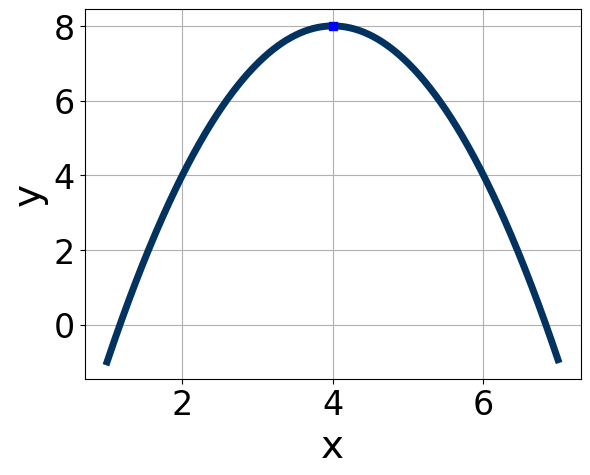
\includegraphics[width=0.5\textwidth]{../Figures/quadraticGraphToEquationC.png}
\end{center}
\begin{enumerate}[label=\Alph*.]
\item \( a \in [-2, 0], \hspace*{5mm} b \in [-12, -7], \text{ and } \hspace*{5mm} c \in [-26, -22] \)
\item \( a \in [0, 4], \hspace*{5mm} b \in [-12, -7], \text{ and } \hspace*{5mm} c \in [24, 25] \)
\item \( a \in [-2, 0], \hspace*{5mm} b \in [7, 9], \text{ and } \hspace*{5mm} c \in [-9, -6] \)
\item \( a \in [0, 4], \hspace*{5mm} b \in [7, 9], \text{ and } \hspace*{5mm} c \in [24, 25] \)
\item \( a \in [-2, 0], \hspace*{5mm} b \in [-12, -7], \text{ and } \hspace*{5mm} c \in [-9, -6] \)

\end{enumerate} }
\litem{
Write the equation of the graph presented below in the form $f(x)=ax^2+bx+c$, assuming  $a=1$ or $a=-1$. Then, choose the intervals that $a, b,$ and $c$ belong to.
\begin{center}
    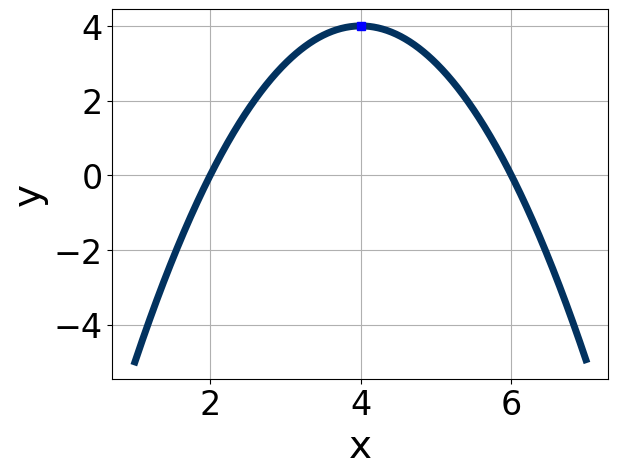
\includegraphics[width=0.5\textwidth]{../Figures/quadraticGraphToEquationCopyC.png}
\end{center}
\begin{enumerate}[label=\Alph*.]
\item \( a \in [-1.6, -0.7], \hspace*{5mm} b \in [5, 11], \text{ and } \hspace*{5mm} c \in [-15, -11] \)
\item \( a \in [-1.6, -0.7], \hspace*{5mm} b \in [-8, -7], \text{ and } \hspace*{5mm} c \in [-15, -11] \)
\item \( a \in [0.3, 2], \hspace*{5mm} b \in [5, 11], \text{ and } \hspace*{5mm} c \in [18, 21] \)
\item \( a \in [-1.6, -0.7], \hspace*{5mm} b \in [-8, -7], \text{ and } \hspace*{5mm} c \in [-22, -19] \)
\item \( a \in [0.3, 2], \hspace*{5mm} b \in [-8, -7], \text{ and } \hspace*{5mm} c \in [18, 21] \)

\end{enumerate} }
\end{enumerate}

\end{document}